\documentclass{article} \usepackage{amsmath} \usepackage{amssymb} \usepackage{amsthm} \usepackage[margin=0.2in]{geometry} \usepackage{hyperref} \usepackage{physics} \usepackage{tikz} \usepackage{mathtools} \mathtoolsset{showonlyrefs} \theoremstyle{definition} \newtheorem{theorem}{Theorem}[section] \newtheorem{corollary}{Corollary}[theorem] \newtheorem{lemma}[theorem]{Lemma} \newtheorem{definition}{Definition}[section] \author{Connor Duncan} \date{\today}
\title{Physics-105-Lecture-Notes-02-14-2019}
\begin{document}
\maketitle\tableofcontents
\noindent\abstract{A single PDF with all lectures in a single document can be downloaded at \url{https://www.dropbox.com/sh/8sqzvxghvbjifco/AAC9LoSRnsRQDp7pYedgWpQMa?dl=0}. The password is 'analytic.mech.dsp'.
 This file was automatically generated using a script, so there might be some errors. If there are, you can contact me at \url{mailto:ctdunc@berkeley.edu}.}
\section{Forced, Damped Oscillators} Try some $F(t)=C_0e^{-i\omega t}$, then we can think about something with a harmonic sollution, i.e. $Z(t)=\tilde{A}e^{-i\omega t}$, with motion described as $\Re{z(t)}$. We punch this into the general solution (homogeneous+inhomogenous), to get an answer.\footnote{Bale said `read the fourier thing' which I assume is a reference to the text} \begin{align} \left(\dv[2]{}{t}+2\beta\dv{}{t}+\omega_0^2\right)z(t)=F(t)/m \end{align} Then, we solve for $\tilde{A}=\frac{C_0}{-\omega_0^2-2i\beta+\omega^2}$. Particular term is complex! \begin{align} \tilde{A}=\frac{\frac{F_0}{m}}{\omega_0^2-2i\beta\omega-\omega^2}=\frac{\frac{F_0}{m}}{\omega_0^2-\omega^2-2\beta i\omega} \end{align} You also get elasitic and absorptive amplitude. \begin{align} A=\frac{F_0/m(\omega_0^2-\omega^2)}{(\omega_0^2-\omega^2)^2+4\beta^2\omega^2}\equiv\text{elastic}\\ B=\frac{2\beta\omega F_0/m}{(\omega_0^2-\omega^2+4\beta^2\omega^2}\equiv\text{absorptive} \end{align} which gives \begin{equation} z(t)=A\cos\omega t+B\sin\omega t+i(B\cos\omega t-A\sin\omega t) \end{equation} \begin{center} 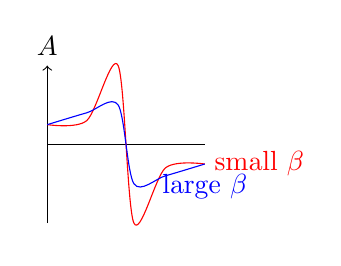
\begin{tikzpicture} \draw(-1,0)--(1,0); \draw[->](-1,-1)--(-1,1) node[anchor=south]{$A$}; \draw[red] plot [smooth] coordinates {(-1,.25)(-0.5,.3)(-.1,1)(.1,-1)(.5,-.3)(1,-.25)} node[anchor=west]{small $\beta$}; \draw[blue] plot [smooth] coordinates {(-1,.25)(-0.5,.4)(-.1,.5)(.1,-.5)(.5,-.4)(1,-.25)}node[anchor=north]{large $\beta$}; \end{tikzpicture} \end{center} constant power$\sim\frac{\text{work}}{\text{time}}$. \begin{align} P(t)=F(t)\cdot\dot z(t)\\ =F_0\cos\omega t\cdot\pdv{}{t}(A\cos\omega t+B\sin\omega t)\\ =F_0\cos\omega t(-\omega A\sin\omega t+\omega B\cos\omega t) \end{align} The first term averages to zero in half a cycle, which is why we call it the elastic amplitude. The average of $B$ over a half cycle represents the energy dissapated by the system, which is the same as $\beta=\frac{1}{2}F_0\omega B$. \begin{equation} \Re(Z)=\frac{A}{\sqrt{(\omega_0^2-\omega^2)+4\beta^2\omega^2}}cos(\omega t-\varphi) \end{equation} With $\varphi=\tan^-1\left(\frac{2\beta\omega}{\omega_0^2-\omega^2}\right)$. \begin{center} 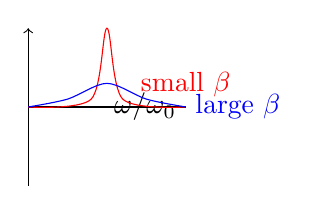
\begin{tikzpicture} \draw(-1,0)--(1,0) node[anchor=east]{$\omega/\omega_0$}; \draw[->](-1,-1)--(-1,1) ; \draw[red] plot [smooth] coordinates {(-1,0)(-0.2,.1)(0,1)(0.2,.1)(1,0)} node[anchor=south] {small $\beta$}; \draw[blue] plot [smooth] coordinates {(-1,0)(-0.5,.1)(0,.3)(0.5,.1)(1,0)} node[anchor=west] {large $\beta$}; \end{tikzpicture} \end{center} Define $Q\equiv$quality factor. \begin{align} Q=\frac{\omega}{2\beta}=\frac{\sqrt{\omega_0^2-\beta^2}}{2\beta}\\ \ddot z+\frac{\dot z}{Q}+z=0 \end{align} Low $Q$ correspond to a lot of damping (i.e. broad resonance), and a high $Q$ corresponds to little damping. Check out Oscillations and Waves by A.P. French. There are also these green functions, which are kind of fun. It's like an optics or quantum problem, when you're crossing a barrier. \begin{align} \ddot z-2\beta\dot z+\omega_0^2z=F_0/m && \text{Region I}\\ \ddot z+2\beta\dot z+\omega_0^2z=0 && \text{Region II} \end{align} You go about solving this using the typical method of solving differential equations, which gives you (in region I) \begin{equation} C_2=\frac{\beta}{m}C_1=\frac{\beta}{\omega_1}\frac{F_0}{m\omega_0^2} \end{equation} Which gives \begin{equation} z(t)=\frac{F_0}{m\omega_0^2}\left[1-e^{-\beta t}\cos\omega_1 t-\frac{\beta}{m}e^{-\beta t}\sin\omega_1 t\right] \end{equation} between $0\leq t\leq\tau$ (boundary). Taylor expanding, we can write this as \begin{equation} z(t) = \frac{F_0}{m\omega_0^2}\left[1-(1-\beta t+\frac{(\beta t)^2}{2}...\right] \end{equation} which simplifies down to \begin{equation} \approx\frac{F_0}{m\omega_0^2}\left(\frac{\omega_0^2 t^2}{2}-\frac{\beta t^2}{2}\right) \end{equation} which tells $z\sim t^2$ for early times, which is about what we'd expect. We also have, at the boundary (a homogeneous solution starting at $t=\tau$). \begin{equation} z_0(t)=e^{-\beta(t-\tau)}\left[D_1\cos\omega_1(t-\tau)+D_2\sin\omega_1(t-\tau)\right] \end{equation} Think of it like integrating over a bajillion little impulses. No testing on green functions apparently (it isn't in the book). \begin{equation} z(t)=\int_{t'\rightarrow-\infty}^tG(t,t')F(t')dt' \end{equation} with $F(t')$ the forcing function, and $G$ the green function. Green function of damped SHO with $z(0)=\dot z(0)=0$: \begin{equation} G(t,t')=\frac{e^{-\beta(t-t')}\sin\omega_1(t-t')}{m\omega_1} \end{equation} DO AT HOME, try taking $F(t')=\alpha t'$ (linearly increasing force), try doing the integral with the forcing function.
\end{document}
